\documentclass{article}

% NeurIPS 2026 workshop CAMERA-READY (TAE / Trust-AI-Eval). De-anonymized:
% the `final' option to neurips_2026 reveals the author block.
% Style file is the unmodified official neurips_2026.sty from
% media.neurips.cc/Conferences/NeurIPS2026/Formatting_Instructions_For_NeurIPS_2026.zip
\usepackage[dblblindworkshop, final]{neurips_2026}
\workshoptitle{TAE (Trust-AI-Eval): Can We Trust AI Evaluation?}

\usepackage[T1]{fontenc}
\usepackage[utf8]{inputenc}
\usepackage{microtype}
\usepackage{graphicx}
\usepackage{booktabs}
\usepackage{amsmath}
\usepackage{amssymb}
\usepackage{amsthm}
\newtheorem{theorem}{Theorem}
\usepackage{url}

\title{Selection-Induced Optimism Can Corrupt Calibration, Not Just Discrimination:
A Code-Verified Audit of Hidden-State Hallucination-Detection Pipelines}

\author{%
  Lakshmi Chakradhar Vijayarao \\
  Northeastern University \\
  Boston, MA, USA \\
  \texttt{vijayarao.l@northeastern.edu} \\
}

\begin{document}
\maketitle

\begin{abstract}
When a checkpoint, layer, threshold, or hyperparameter is selected on data
later reused to report performance, the reported number is optimistic. This is
well documented for \emph{discrimination} metrics such as AUROC. \emph{In the
settings we test}, the same selection step also corrupts \emph{calibration} --
how reliable a system's stated confidence is, not just how well it ranks --
and degrades the operating point a selective-prediction threshold is believed
to buy. Selecting one layer by argmax over $32$ candidates, with no fitting on
the evaluation data at all, inflates achieved risk by $10$--$16\%$ relative to
the believed budget: at a $70\%$ coverage \emph{target} over $100{,}000$
queries a day, $1{,}082$ additional unflagged errors daily (BCa $95\%$
$[435,1718]$), priced at the coverage each arm actually achieves because the
transferred threshold does not preserve coverage.
We separate calibration from discrimination rather than inferring it: under a
Murphy decomposition the \emph{reliability} term carries the effect
($+0.0046$, BCa $[+0.0027,+0.0065]$) while \emph{resolution} does not
($+0.0028$, covering zero). The ECE gap holds in all eight binning settings
(four bin counts, equal-width and equal-mass) and a binning-free calibration
slope agrees ($0.68$ reused versus $0.62$ held out). A placebo at prespecified
rather than selected layers shows roughly \emph{half} the gap is
selection-specific and half ordinary reuse; we report both. A second,
structurally different mechanism and a real
ECE bug in an externally published, pinned-commit-verified pipeline corroborate
the direction. Nine of ten cells are established per-cell -- six cleanly,
three resting on a non-negativity our own method section disqualifies -- and
all nine survive family-wise correction. Regularization does not explain the
effect -- at a probe that cannot interpolate the increment grows -- but a
second harness bounds it: on real features from two model families, selection
inflates discrimination ($+0.007$ AUROC, established in both) \emph{without}
corrupting calibration.
Measured severity is a property of a (mechanism, metric, control)
\emph{triple}: one cell spans $1.44\times$ across two admissible controls. We
release the taxonomy, three pinned third-party verifications, a checklist
extending Kapoor \& Narayanan and REFORMS, and a negative result -- a regex
scanner automating four of its five items finds zero true positives across
seven repositories and misses both leaks it was built to catch. Our object of
study is the evaluation protocol, not the model.
\end{abstract}

\section{Introduction}

The protocol we study is
hidden-state probing for hallucination detection: a linear probe is cheap to
train, and reported AUROCs are often striking -- $0.90$ or higher, sometimes a
perfect $1.000$ -- in a regime of few samples and many dimensions, where such
numbers should invite scrutiny of the procedure that produced them.

Work that has scrutinized this protocol (adaptive data analysis,
post-selection inference, and this paper's own prior audit) measures its effect
on \emph{discrimination}: does a selection-biased AUROC overstate how well a
probe ranks hallucinated versus correct generations? The closest audit in this
paradigm, on a different detection task, scopes calibration out explicitly:
Li et al.\ (2026, \S5.2) report AUC only, stating that ``calibration is not the
target estimand.'' To our knowledge no prior audit of this failure class has asked whether the
same selection step also corrupts \emph{calibration}. We show that it can, and
measure where it does not: a probe
scored at its own selected configuration on the data used to select it yields
Brier and ECE values that look better than its genuinely held-out reliability,
with the same statistical signature (BCa-established, excluding zero) as the
discrimination gap this literature already distrusts. We confirm it under two
unrelated causes -- our own bridge experiments
(\S\ref{sec:calibration-bridge}) and a real bug in an external pipeline's
reported metric (\S\ref{sec:mechanism5-ece}) -- because it changes what
auditing must check: \textbf{a clean AUROC does not imply a clean confidence
estimate}, and a practitioner who checks only discrimination can still deploy
a probe whose reported reliability is an artifact of selection.

Our second claim is that measuring this bias is harder than it looks: its
apparent size depends on which control the reported number is compared against,
not only on which mechanism produced it. A single case-study cell spans
$1.44\times$ across two admissible controls (\S\ref{sec:related}) --
severity is a property of a (mechanism, metric, \emph{control}) \emph{triple}.

A nested-cross-validation leakage bug in a probing pipeline we had full
commit-history access to provided the seed case for this taxonomy; the
question it raised -- isolated or structural -- defines the paper's scope. We identify five \emph{distinct} mechanisms by
which evaluation labels leak into a reported metric, verify three against
pinned commits of externally published pipelines, and measure each against a
matched control (\S\ref{sec:mechanisms}); most are small on the AUROC scale,
one is not. A self-audit turns the same scrutiny on our own work: Mechanism 3's
primary synthetic estimate does not survive correction for its own
construction asymmetries.

\paragraph{Contributions.}
\begin{itemize}
\itemsep0pt
\item The first evidence that selection-induced optimism \emph{can} corrupt
   calibration and degrade an actual selective-prediction operating
   point, not only discrimination: confirmed on two mechanisms
   (\S\ref{sec:calibration-bridge}), a structurally different external
   confirmation (\S\ref{sec:mechanism5-ece}), and an operational
   consequence -- a $10$--$16\%$ relative inflation of a deployed error
   budget from a single argmax over candidate layers
   (\S\ref{sec:selective-prediction}).
\item A five-mechanism taxonomy of label-information leakage specific to
   hidden-state probing pipelines, three verified directly against pinned
   third-party source code (\S\ref{sec:mechanisms}).
\item The within-harness severity relationship (diagnostic, not predictive:
   $9.2$--$24.3\times$ off on matched real-feature measurements) and a
   matched comparison licensing only a negative conclusion about mechanism
   identity's contribution beyond candidate count and operating point
   (\S\ref{sec:severity}).
\item Two findings from turning our own methods on themselves: a quantified
   CV-based layer-selection optimism bias, and a factorial decomposition
   showing our own primary severity estimate fails its own correction.
\item A checklist synthesizing all five mechanisms into actionable questions,
   extending the Kapoor \& Narayanan and REFORMS leakage checklists, plus a
   negative automation result diagnosed rather than generalized from
   (\S\ref{sec:checklist}).
\end{itemize}

\paragraph{What each claim is, and how strongly.} Every claim sits in one tier
of Table~\ref{tab:tiers}, read at that tier and nowhere at a stronger one;
Appendix~\ref{app:claim-tiers} assigns every individual result to one.

\begin{table}[h]
\centering
\small
\vspace{-0.6em}
{\setlength{\tabcolsep}{4pt}
\begin{tabular}{@{}p{0.15\linewidth}p{0.80\linewidth}@{}}
\toprule
\textbf{A} Documented & Present in the harness as written; descriptive, no effect size claimed. Five mechanisms, three traced to pinned third-party source. \\
\textbf{B} Established & BCa $95\%$ excludes zero, Holm-corrected where a family applies. M2's discrimination, calibration and operating-point results; M1/M3/M5 severities. \\
\textbf{C} Illustrative & Reported, not relied on. Our primary synthetic estimate (fails its own control), a non-reproducible prior number, and the scope limits including a negative cross-harness calibration result. \\
\bottomrule
\end{tabular}}
\caption{How to read every claim here. No prevalence estimate is given:
repositories were found by targeted search, not sampled.}
\label{tab:tiers}
\end{table}


\begin{figure}[t]
\centering
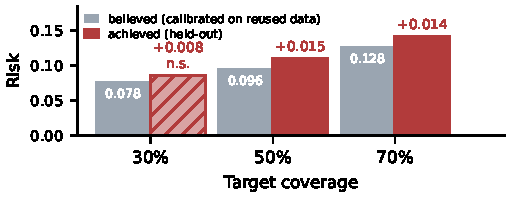
\includegraphics[width=0.52\linewidth]{figures/fig1_risk_coverage.pdf}
\caption{The consequence, before any mechanism-level detail. Grey is the
selective-prediction risk a practitioner believes they bought by calibrating
on reused data; red is what is incurred on held-out data at the identical
threshold -- $10$--$16\%$ of the target risk, or $1{,}082$ unflagged errors a
day per $100{,}000$ queries at a $70\%$ coverage target, each arm priced at the
coverage it actually achieves. The $30\%$ cell is hatched: its BCa interval on
the risk difference covers zero. \textbf{The selected object is a single
integer}, which of $32$ layers to report (Mechanism~2,
\S\ref{sec:selective-prediction}).}
\label{fig:risk-coverage}
\end{figure}

\section{Related Work}
\label{sec:related}

\paragraph{Calibration, selective prediction, and conformal prediction.}
Our calibration-bridge finding (\S\ref{sec:calibration-bridge}) connects
selection bias to the calibration literature (Guo et al., 2017) and, via
\S\ref{sec:selective-prediction}, to selective prediction (Geifman \&
El-Yaniv, 2017), which formalizes the risk-coverage tradeoff we use.
Conformal prediction (Angelopoulos \& Bates, 2023) and risk-controlling
prediction sets (Bates et al., 2021) formally treat the question
\S\ref{sec:selective-prediction} asks informally -- does a threshold
calibrated on one sample control risk on another. We illustrate that question
on selection-biased scores rather than proving a new risk-control result: those
raw scores are themselves corrupted by the selection step audited here, a risk
any conformal wrapper built on them inherits unchecked. To our knowledge none
of these literatures has been connected to the leakage mechanisms in
\S\ref{sec:mechanisms}.

\paragraph{The definition we use.} \emph{Leakage is a change in the
expectation of a reported metric attributable to evaluation-target
information entering the estimation process.} The change is
\emph{control-relative}: severity is not a (mechanism, metric) \emph{pair}
but a (mechanism, metric, control) \emph{triple} -- the difference between
the leaky procedure and \emph{some} counterfactual, and defensible
counterfactuals disagree. On one Mechanism-3 cell the two defensible
controls -- a blind retrain on the full fold, and the same retrain on the
$85\%$ subset its epoch count was chosen on -- give $+0.0034$ and $+0.0049$,
a $1.44\times$ spread; a contaminated adaptive control we disqualify on
independent grounds gives $+0.0198$, making it $5.8\times$.

\paragraph{Adaptive data analysis and post-selection inference.} Two of our
five mechanisms -- select a layer or threshold on the test set, then report at
that choice -- are the canonical setting of adaptive data analysis (Dwork
et al., 2015). Our candidate-count relationship (\S\ref{sec:severity}) is
shape-consistent with that bound, whose worst-case guarantees exceed every
severity we measure by two to three orders of magnitude. Cawley \& Talbot (2010) show
model-selection over-fitting induces bias growing with candidate count --
Mechanism 2's failure mode; new here is that the selected object is a layer
index of a frozen network, contaminating a localization claim, not only a
number. Both mechanisms have canonical priors outside ML (Ambroise \&
McLachlan, 2002; Varma \& Simon, 2006, with nested CV as the remedy), and we
claim no novelty on either discrimination result. What is new here is that the
same two selection steps corrupt \emph{calibration} and degrade the realized
risk of a selective-prediction rule at a transferred threshold -- an estimand
neither line of work measures.

\paragraph{Existing leakage taxonomies and contamination.} The closest
prior art is Kapoor \& Narayanan (2023, an 8-type taxonomy across 17
fields) and REFORMS (Kapoor et al., 2024, a 32-item checklist); Mechanism 1 is a direct case of
their L1.3, feature selection under test-set visibility; Mechanism 4 applies
the same structure to a layer index. The remaining three select against a
validation signal rather than across the train/test boundary, and map onto
neither taxonomy, since both
treat train/test separation as the leakage surface, not iterative model
selection against a validation signal. Roth (2026) quantifies four leakage
classes across 2,047 datasets, but in discrimination only. Hussain \& Kantarcioglu (2026, PARALLAX) find
four of six corpora leak the ground-truth answer directly into the prompt,
via a mechanism distinct from all five here; pretraining-data contamination
(Shi et al., 2024) is different still: what the model has already seen,
not whether a selection step used test-set signal afterward.

\section{Method}
\label{sec:method}

Two case studies come from our own prior work, with full code, data, and
commit-history access. The external ones required a real, runnable public
repository verified via the host, a reported AUROC $\geq 0.90$, and an
evaluation protocol whose leakage risk we could assess from the code.

\paragraph{Evidentiary status.} Three case studies are \emph{fully verifiable
here} -- checkpoint selection (MultiHaluDet), best-layer selection
(HallucinationPatternDetection), and test-set threshold selection
(Mechanism 5, audited in \emph{both} of the above repositories at the same
pinned commits) -- all external, published, code-available systems,
with every script and result JSON released; the third is detailed with its
calibration-contamination bug in \S\ref{sec:mechanism5-ece}. One (CV-based
layer selection) is \emph{verifiable from a derived artifact}: our own prior
pipeline, whose raw hidden-state cache is too large to ship, though a small
derived artifact lets a reader recompute the primary numbers. One
(full-dataset probe reuse) is \emph{not independently re-verifiable} -- its
number comes from our own prior work with no surviving scripts; we keep it
because the mechanism is real and is this paper's origin, but never compare it
against the code-verified numbers.

\paragraph{Severity is not one scale.} Four named quantities avoid
conflation: $\Delta_{\text{synth}}$ (calibrated synthetic-harness gap at a
fixed Bayes-optimal operating point), $\Delta_{\text{real}}$ (the same on
real Mistral-7B/HaluEval features), $\Delta_{\text{sel}}$ (within-split
selection-specific component against its own permutation null), and
$\Delta_{\text{boot}}$ (bootstrap max-bias over already-published AUROC
arrays, no model retrained) -- all AUROC differences, sharing units but not
a reference. BCa (bias-corrected and accelerated bootstrap) 95\% intervals
are the default decision rule (established
when the interval excludes zero) except for one case study, whose two
candidate estimators are provably non-negative by construction, exactly the
condition under which BCa's correction cannot restore coverage (simulation
confirms $0\%$ empirical coverage there), so we never use BCa as evidence
for that case study.

\paragraph{Multiple-comparison correction.} Where we additionally compute
Holm-Bonferroni across cells tested together (Table~\ref{tab:holm}), it
eliminates the marginal finding in most families we checked.
Applying family-wise control, no marginal finding survives outside
one mechanism's non-marginal threshold-selection result (a single large
effect outside any multi-cell family) and the table's exceptions (two
families, three cells).


\section{Five Mechanisms, Measured}
\label{sec:mechanisms}

Three axes locate the five mechanisms: (a) the provenance of the statistic
selected on -- full-dataset labels, an inner CV fold, or the test set; (b)
the object selected -- a feature, a layer, a checkpoint, or a threshold; and
(c) whether the selection's output is reused downstream as a feature. These
are documented instances, not an orthogonal partition.


Table~\ref{tab:severity} (Appendix~\ref{app:severity}) gives every
mechanism's severity traced to source code, one row per mechanism (two each for Mechanisms 1 and 3, whose harnesses disagree
or differ in provenance). Mechanism 1's narrative number ($+0.19$, from prior
work) is excluded from every cross-mechanism comparison and shown only for
orientation; its \emph{second} row is a new controlled synthetic
reconstruction that \emph{is} code-verified and is $5.1$--$11.4\times$
above every Mechanism 2--4 estimate. Every cross-mechanism severity comparison in this
paper pools only Mechanisms 2--4.



\paragraph{Two numbers are as much about measurement as about leakage.}
Mechanism 3's \emph{primary} synthetic estimate does not survive its own
control: a $2\times2\times2$ factorial crossing selection-set size,
selection-run budget, and training depth carries the as-published control's
$+0.0030$ to a fully corrected $-0.0001$ (BCa $[-0.0021,+0.0021]$,
$p=0.657$), attributing $75.5\%$ of the movement to selection-set size at the
shipped early-stopping fraction -- a dominant factor, not a fixed one
(Appendix~\ref{app:resampling}).
The decomposition, not the null, is the contribution: it names the
construction choice that manufactures a false positive of this size.
Mechanism 4's estimate rests on a statistic non-negative by construction
(Appendix~\ref{app:nonneg} states and proves both), so its sign carries no
information; against a permutation null, no cell is significant above it.
Mechanism 5's F1 severity is $n$-dependent ($\approx6.3\times$ smaller at
$n{=}2000$ vs.\ $n{=}140$); whether it stays distinguishable from noise at
typical benchmark sizes is untested here.

\section{What Governs Severity Within a Harness}
\label{sec:severity}

Within one harness, severity rises monotonically and concavely with candidate
count $K$ at a fixed operating point, from $+0.0093$ at AUROC$_0=0.70$ to
indistinguishable from zero at $0.985$ ($p=0.219$, $n=100$). This
$K$-regularity is scoped to checkpoint-along-a-trajectory candidates only: an
independently-seeded, exchangeable-candidate replication at adequate power
($N=200$) does not reproduce it (gaps $+0.0013$ to $-0.0010$, every CI covering
zero). The operating-point relationship is not similarly scoped but does not
transport across harnesses -- it is exceeded by roughly an order of magnitude
at a matched operating point in our own real-feature harnesses.

\paragraph{Does mechanism identity matter beyond these two covariates?} A
matched comparison at a common $(K,\text{AUROC}_0)$ shows a
per-mechanism-intercept model beats a pooled one decisively ($304\times$
intercept spread), and a pooled fit without a mechanism term gives a
wrong-signed $\ln K$ coefficient that flips once mechanism is controlled for.
Some factor beyond candidate count and operating point is not absorbed by them
-- though this design cannot separate whether it is mechanism identity itself
or the unequal harness maturity correlated with it. What this licenses is only
the negative conclusion: severity is not governed by those two covariates to
the exclusion of mechanism.

\section{Operational Consequences: Selection Bias Degrades Selective Prediction}
\label{sec:calibration-bridge}

A selective-prediction threshold calibrated on reused-fold scores buys a risk
budget the deployed system does not meet
(Table~\ref{tab:selective-prediction}): choosing one of $32$ layers by argmax
inflates it by $10$--$16\%$ relative. This is the paper's most robust
finding at the $50\%$-coverage point tested for regularization: it survives a
check the raw calibration gap driving it does not
(\S\ref{sec:selective-prediction}). We first show why, then that it is not
limited to one construction.


Every severity number so far is a gap in AUROC or F1 -- discrimination
metrics, which ask only whether a probe ranks positives above negatives
correctly. None of them ask whether the probe's \emph{probability outputs}
are honestly reliable: whether a prediction made at $0.9$ confidence is
right about $90\%$ of the time. This is a different question, and the
literature on selection bias in evaluation (adaptive data analysis,
post-selection inference, and this paper's own \S\ref{sec:mechanisms}) has
not asked it for this failure class. We do, on two structurally distinct
mechanisms already audited above, using their own already-computed scores --
no new data, no new model calls, only a new metric applied to existing
LEAKY/CLEAN\_MATCHED comparisons (defined below).

\paragraph{Method.} For Mechanism 2 (CV-argmax layer selection), we take the
CV-selected layer's own probability outputs on the reused selection fold
(LEAKY) against the same layer's probability outputs on the genuinely
held-out split (CLEAN\_MATCHED), across the same 50 randomized-split
repetitions \S\ref{sec:mechanisms} already uses, replicating that section's
layer-selection rule exactly (verified: selected layers match to the rep).
For Mechanism 1's real-feature analog, we take the same full-dataset-fit
probe's in-sample probability outputs (LEAKY) against a 5-fold
out-of-fold refit (CLEAN\_MATCHED), on the same cached real Mistral-7B/HaluEval
features and probe convention as its AUROC comparison (replication verified
to four decimal places against that AUROC number). For both, we report Brier
score (primary; well-defined without binning at these sample sizes) and
10-bin expected calibration error (ECE; secondary, standard in the
calibration literature), with the same BCa 95\% bootstrap interval this
paper uses throughout.

\begin{table}[t]
\centering
\small
{\setlength{\tabcolsep}{3pt}
\begin{tabular}{@{}p{0.26\linewidth}p{0.33\linewidth}p{0.33\linewidth}@{}}
\toprule
Mechanism & Brier gap (BCa 95\%) & ECE gap (BCa 95\%) \\
\midrule
2 (CV-argmax layer selection) & $+0.0082$ \newline $[+0.0030,+0.0137]$ & $+0.0171$ \newline $[+0.0099,+0.0242]$ \\
1 (full-dataset probe reuse, real features) & $+0.0260$ \newline $[+0.0252,+0.0269]$ & $+0.0193$ \newline $[+0.0184,+0.0203]$ \\
\bottomrule
\end{tabular}}
\caption{Calibration gap (CLEAN\_MATCHED minus LEAKY; positive means the
leaky condition looks more reliable than it honestly is). Mechanism~2:
$50$ randomized splits, from a cached pipeline whose raw hidden-state cache is
too large to ship, though a derived artifact lets a reader recompute these
numbers. Mechanism~1: $n{=}400$, computed on the cached
real-feature analog -- \emph{not} the non-reproducible prior-work number of
\S\ref{sec:method}, which is excluded here as everywhere. All four cells
survive Holm-Bonferroni jointly with Table~\ref{tab:selective-prediction}.}
\label{tab:calibration-bridge}
\end{table}

\paragraph{Result.} Both gaps are positive and both intervals exclude zero
for both mechanisms (Table~\ref{tab:calibration-bridge}). Mechanism 2 carries
the claim: an argmax over $32$ candidate layers, with no fitting on the
evaluation data at all, still moves Brier by $+0.0082$ and ECE by $+0.0171$, both
BCa-established. \textbf{Both replicate on a disjoint
HaluEval pool of the same size} ($+0.0112$ and $+0.0200$, each established
and larger); both pools are Mistral-7B, so the \emph{calibration} gap is
established across question sources on one model, and the selection step
itself across architectures next.

\paragraph{Is it calibration, and is it selection?} Three checks on the same
$50$ splits; full tables in Appendix~\ref{app:reviewer-response}.
\emph{(i)} A Brier gap mixes calibration with discrimination, which
argmax-AUROC optimises directly, so it cannot on its own carry a calibration
claim. Under $\mathrm{BS}=\mathrm{REL}-\mathrm{RES}+\mathrm{UNC}$ the
\textbf{reliability} term carries the effect ($+0.0046$, BCa
$[+0.0027,+0.0065]$) and \textbf{resolution} does not ($+0.0028$, covering
zero); base rates are matched, so uncertainty contributes $+0.0009$. Two
binning-free statistics agree -- calibration slope $0.6807$ to $0.6185$, smooth
calibration error $+0.0034$ (BCa $[+0.0020,+0.0050]$) -- so we rest the
calibration claim on reliability and read Brier as a degradation in
probabilistic prediction quality.
\emph{(ii)} The ECE gap survives all eight binning settings (bin count
$\in\{5,10,15,20\}$, equal-width and equal-mass), spanning $+0.0164$ to
$+0.0212$ with the submitted $+0.0171$ mid-range.
\emph{(iii)} Repeating the comparison at unselected layers gives a real but
smaller placebo (reliability $+0.0020$), so \textbf{roughly $57\%$ of the gap
is selection-specific and $43\%$ ordinary reuse} (increment $+0.0026$, BCa
$[+0.0014,+0.0040]$; ECE $+0.0099$, BCa $[+0.0054,+0.0150]$). Both components
are established and we claim only the increment for selection. Resolution's
increment is \emph{negative} ($-0.0048$, BCa $[-0.0066,-0.0031]$), as expected
if selection buys in-sample discrimination, and is a second reason not to read
Brier as the calibration result.

\paragraph{Across architectures, and scope.} Re-running the argmax protocol on
cached states from four other architectures -- identical $n$, split, folds,
reps, seed and probe -- the selection-specific component is positive on all
four and established on three (per-architecture values in
Appendix~\ref{app:reviewer-response}); Qwen-7B is not, at $\alpha{=}0.05$.
\textbf{The sign carries; significance and magnitude do not.} Those caches are
forced-choice rather than generation-labeled, so task and architecture change
together and we attribute the difference to neither alone; they test the AUROC
selection component, not calibration. Mechanism 1's larger gap ($+0.0260$
Brier) follows from its degenerate construction, not from selection; its probe
interpolates at $C{=}1.0$ and \textbf{its ECE gap does not survive} $C{=}0.01$,
where Mechanism 2's increment does (Appendices~\ref{app:reg},
\ref{app:regularization}). We establish calibration on two of the five
mechanisms and on one feature representation: run on real features from two
model families, this same construction inflates discrimination \emph{without}
corrupting calibration (Appendix~\ref{app:secondfamily}). \textbf{The
calibration consequence does not follow automatically from the discrimination
one}, and where it does hold, the selection step that inflates AUROC also makes
the resulting confidence estimates look more trustworthy than they are.

\subsection{Does this move a deployment's actual error budget?}
\label{sec:selective-prediction}

A calibration gap alone leaves open whether it has operational stakes. We
use the selective-prediction framework (fix a confidence threshold, abstain
below it, and rely on the error rate among non-abstained predictions) to
check directly: if a practitioner calibrates a deployment threshold using
the same reused-fold (LEAKY) scores this paper already shows are optimistic,
what risk do they actually get when that identical threshold is applied to
genuinely new (CLEAN\_MATCHED) data?

\paragraph{Method.} At each of three target coverage levels ($30\%$, $50\%$,
$70\%$) we take the threshold achieving that coverage on LEAKY and LEAKY's own
reported risk there -- what a practitioner using only the reused fold would
believe -- then apply the identical numeric threshold to CLEAN\_MATCHED. Risk
violation is actual minus believed, BCa $95\%$ as elsewhere.

\begin{table}[t]
\centering
\small
{\setlength{\tabcolsep}{3pt}
\begin{tabular}{@{}p{0.08\linewidth}p{0.13\linewidth}p{0.13\linewidth}p{0.12\linewidth}p{0.32\linewidth}@{}}
\toprule
Mech. & Cover-\newline age & Believed risk & Actual risk & Violation (BCa 95\%) \\
\midrule
2 & 30\% & 0.078 & 0.086 & $+0.008$ $[-0.001,+0.018]$ \emph{(n.s.)} \\
2 & 50\% & 0.096 & 0.110 & $+0.015$ $[+0.007,+0.023]$ \\
2 & 70\% & 0.128 & 0.142 & $+0.014$ $[+0.005,+0.023]$ \\
1 & 30\% & $0.000$ & 0.002 & $+0.002$ $[+0.001,+0.004]$ \\
1 & 50\% & $0.000$ & 0.007 & $+0.007$ $[+0.006,+0.008]$ \\
1 & 70\% & $0.000$ & 0.009 & $+0.009$ $[+0.008,+0.010]$ \\
\bottomrule
\end{tabular}}
\caption{Selective-prediction risk violation: risk a practitioner believes
they have (from LEAKY) versus risk actually achieved (on CLEAN\_MATCHED) at
the identical threshold ($n$ as in Table~\ref{tab:calibration-bridge}). The
violation column is the paired per-split mean, so it need not equal the
difference of the two rounded risk columns. These six rows and
Table~\ref{tab:calibration-bridge}'s four form one $10$-cell family; nine are
established per-cell and all nine survive Holm-Bonferroni correction.
\textbf{Three of the nine rest on a construction we disqualify elsewhere}:
Mechanism 1's believed risk is exactly zero, so its violation \emph{is} the
achieved risk -- non-negative by construction, where \S\ref{sec:method}
declines BCa as evidence. \textbf{Six carry no such caveat.}}
\label{tab:selective-prediction}
\end{table}

\paragraph{Result.} \textbf{Mechanism 2 carries this result}, and it is the
harder case: the only quantity chosen on the reported data is a single
integer, which of $32$ layers to use. Its violation is established at $50\%$ and
$70\%$ coverage and not at $30\%$, where the BCa interval covers zero before
any correction -- a $10$--$16\%$ relative inflation of the target risk.

\paragraph{Pricing the transfer at the coverage actually achieved.} A threshold
chosen for a $70\%$ coverage \emph{target} on the reused fold does not deliver
$70\%$ coverage once the score distribution shifts; it delivers $70.71\%$.
Multiplying a risk difference by a fixed answered-query count therefore
misprices the transfer, so we price each arm at the coverage it achieves. At a
$70\%$ target a practitioner has bought $0.128$ risk over the $70{,}000$
queries they expect to answer, or $8{,}945$ errors; the system answers
$70{,}707$ at $0.142$, or $10{,}027$ -- \textbf{$1{,}082$ additional unflagged
errors daily} (BCa $[435,1718]$), against $972$ under the fixed-coverage
estimator, and $825$ at $50\%$. Coverage shifts furthest at the $30\%$ target,
where the coverage-aware excess of $368$ errors excludes zero, $[77,662]$,
and the fixed-coverage estimator's does not; we flag that cell as established
\emph{only} under the coverage-aware count and keep the risk-difference
verdict as the conservative one (Appendix~\ref{app:reviewer-response}). What
degrades is the abstention rate a deployment was sized against; this transfers
an empirically chosen threshold and neither constructs nor contradicts a
distribution-free risk-controlling procedure. The per-day counts scale one
dataset's split-to-split behaviour to a hypothetical query volume: they convey
magnitude, not a population estimate.

\paragraph{Mechanism 1, and robustness.} With a candidate set of size one,
selection reduces to fitting on the evaluation data: believed risk is
\emph{exactly zero} at every coverage against an actual $0.2$--$0.9\%$. That is
the largest cell in the paper and the least informative -- non-negative by
construction, not independent of \S\ref{sec:calibration-bridge}'s Brier gap,
and an already-documented error -- so we retain it as the degenerate case the
other four are weaker versions of and base no claim on it. Repeating the
analysis at $C=0.01$, away from exact interpolation, leaves the risk violation
intact ($+0.0079$, BCa $[+0.0070,+0.0090]$ at $50\%$, against $+0.0075$ at
$C=1.0$ -- if anything marginally larger). The consequence therefore does not
depend on the near-interpolation regime that shrinks the raw Brier/ECE gaps,
unlike the raw calibration-gap magnitude, which does.

\subsection{An independent confirmation: ECE contamination verified in the audited pipeline itself}
\label{sec:mechanism5-ece}

Unlike \S\ref{sec:calibration-bridge}'s Mechanisms 1/2 findings --
LEAKY/CLEAN\_MATCHED comparisons we construct on our own cached scores -- this
is a bug we \emph{found} in MultiHaluDet's own code (a multilingual
hallucination-detection pipeline; Alvi et al., 2026; pinned commit
\texttt{c759751}). Its ECE term uses
\texttt{confidence=max(probs,1-probs)} (threshold-independent) but
\texttt{correct=(preds==labels)}, with \texttt{preds} thresholded at Mechanism
5's own test-label-selected Youden cut: \textbf{the pipeline's own reported ECE
is contaminated by the mechanism this paper audits it for.} Quantified with the
already-validated Mechanism-5 synthetic harness (Appendix~\ref{app:ece}), the
pooled ECE gap across five operating points is $+0.0090$, all five cells
BCa-established and Holm-Bonferroni-surviving. The accompanying Wilcoxon
statistics index the harness's seed-to-seed reproducibility, not the deployed
pipeline, and we do not read them as the latter.

This is verified in one of the two audited Mechanism-5 repositories, and we do
not generalize from one instance. Its value is structural: it shows the pattern
under a cause unrelated to Mechanisms 1/2's near-in-sample separation, so the
pattern is not only a memorization artifact. Taken with
\S\ref{sec:calibration-bridge}, that is \emph{two} independent confirmations,
not three, converging in direction and not in magnitude.

\section{A Checklist for This Literature}
\label{sec:checklist}

Five questions cover the five mechanisms above, in checklist rather than
taxonomy order (full version with per-item fixes in supplementary material):

\begin{enumerate}
\itemsep0pt
\item (M1) Is any feature computed by fitting on the full dataset's labels
   before an outer CV loop treats part of that dataset as held out?
\item (M3) Inside a CV fold, is a ``best'' checkpoint/epoch chosen on the same
   fold whose predictions are reused downstream as clean out-of-fold output?
\item (M4) Is a ``best'' layer/config selected by argmax of a metric computed
   on the same test set later reported as the headline number, across many
   candidates, with no correction?
\item (M2) Was a hyperparameter chosen by maximizing a cross-validated metric,
   with that same CV number reported as performance and no genuinely held-out
   check?
\item (M5) Was a decision threshold chosen by optimizing a metric on the test
   labels themselves, with that same test set used to report the metric at
   that threshold?
\end{enumerate}

Q1--Q5 name the mechanism and where to look; three are pinned-commit-verified.
Q5 catches what nothing upstream will: AUROC ignores threshold selection, so an
AUROC-only audit misses inflated F1/accuracy. The checklist supplies no
severity \emph{number} -- \S\ref{sec:severity}'s surface is not a calculator
(matched measurements exceed its prediction by $9.2$--$24.3\times$). Measure
severity in your own harness against a matched control.

\paragraph{Is the checklist automatable by static analysis?} Not at the line
level, and the failure mode is diagnostic. A regex scanner for four of the five
patterns, run against 7 repositories (2 audited, 5 externally found), produced
7 raw hits, all false positives on manual reading, and missed both known true
positives -- a keyword-list gap, and an argmax-plus-test-variable design that
cannot fire when the test split lives in another module. A blinded
language-model re-read agreed with all 7 classifications and located both
missed bugs unprompted. Line-level regex matching is the wrong tool: selection
statements relate to what they select on, often across files -- not evidence
the class resists static detection.

\paragraph{The prescribed fixes are cheap.} Nesting cross-validation removes
$+0.0232$ AUROC of Mechanism 2's optimism (one run, within 1 SD of
Table~\ref{tab:severity}'s $+0.0255$) in seconds of CPU time; constructing
Mechanism 3's control fairly -- matching the honest arm's selection-set size to
LEAKY's, worth $75.5\%$ of the $+0.0030\to-0.0001$ movement against $28.1\%$
for the disjoint held-out set -- costs under 5 minutes, with a
$+0.0006$--$+0.0030$ residual surviving on real features. Both are measured
against their naive alternatives, not merely prescribed.

\section{Conclusion}

Selection-induced optimism corrupts calibration, not only discrimination
(\S\ref{sec:calibration-bridge}--\ref{sec:mechanism5-ece}), under two unrelated
causes and unmeasured before for this failure class: a clean discrimination
metric does not imply a clean confidence estimate. The five-mechanism taxonomy
is the most reusable artifact here, pending a prevalence study not run.

We held this paper to the standard it asks of the literature it audits, and
report the cost: our own primary severity estimate does not survive its own
correction, we decline BCa where the estimator makes it invalid, and where a
robustness check split our findings we report all outcomes. An audit of
evaluation protocols that exempts itself measures nothing.

\section*{Limitations}

Calibration is established on two of five mechanisms and one feature
representation; roughly half of even that gap is ordinary reuse rather than
selection, and on real features from two model families the selection-specific
calibration increment is null or negative
(Appendix~\ref{app:secondfamily}). Mechanism 1's ECE gap does \emph{not}
survive regularization, though Mechanism 2's increment does. We give no
prevalence estimate, the severity surface is a fit rather than a bound, and one
case study's headline number is not independently re-verifiable.
Appendices~\ref{app:prevalence}--\ref{app:limitations} have the rest.

\section*{References}

Alvi, R., Sayeedi, N. L., \& Sayeedi, M. F. A. (2026). MultiHaluDet:
Multilingual Hallucination Detection via LLM Hidden State Probing. In
\emph{Proceedings of the 1st Workshop on Multilinguality in the Era of
Large Language Models (MeLLM 2026)}.

Ambroise, C., \& McLachlan, G. J. (2002). Selection Bias in Gene Extraction on
the Basis of Microarray Gene-Expression Data. \emph{Proceedings of the National
Academy of Sciences}, 99(10), 6562--6566.

Angelopoulos, A. N., \& Bates, S. (2023). Conformal Prediction: A Gentle
Introduction. \emph{Foundations and Trends in Machine Learning}, 16(4).

Bates, S., Angelopoulos, A., Lei, L., Ryan, J., Malik, J., \& Jordan, M.
(2021). Distribution-Free, Risk-Controlling Prediction Sets. \emph{Journal
of the ACM}, 68(6).

Cawley, G. C., \& Talbot, N. L. C. (2010). On Over-fitting in Model
Selection and Subsequent Selection Bias in Performance Evaluation.
\emph{Journal of Machine Learning Research}, 11, 2079-2107.

Dwork, C., Feldman, V., Hardt, M., Pitassi, T., Reingold, O., \& Roth, A.
(2015). Preserving Statistical Validity in Adaptive Data Analysis.
\emph{Proceedings of the 47th Annual ACM Symposium on Theory of Computing
(STOC 2015)}.

Ezharjan [GitHub handle; author name not stated in the repository]
(2026). HallucinationPatternDetection: Hallucination Pattern
Detection in Open-Source LLMs [Software]. GitHub repository, commit
\texttt{ea0b967}.
\texttt{github.com/Ezharjan/\allowbreak HallucinationPatternDetection}.

Geifman, Y., \& El-Yaniv, R. (2017). Selective Classification for Deep
Neural Networks. \emph{Advances in Neural Information Processing Systems
(NeurIPS 2017)}.

Guo, C., Pleiss, G., Sun, Y., \& Weinberger, K. Q. (2017). On Calibration
of Modern Neural Networks. \emph{International Conference on Machine
Learning (ICML 2017)}.

Hussain, K., \& Kantarcioglu, M. (2026). PARALLAX: Separating Genuine
Hallucination Detection from Benchmark Construction Artifacts.
arXiv 2605.17028.

Kapoor, S., \& Narayanan, A. (2023). Leakage and the Reproducibility
Crisis in ML-based Science. \emph{Patterns}, 4(9). arXiv 2207.07048.

Kapoor, S., Cantrell, E. M., Peng, K., Pham, T. H., Bail, C. A., Gundersen,
O. E., Hofman, J. M., Hullman, J., Lones, M. A., Malik, M. M., Nanayakkara, P.,
Poldrack, R. A., Raji, I. D., Roberts, M., Salganik, M. J., Serra-Garcia, M.,
Stewart, B. M., Vandewiele, G., \& Narayanan, A. (2024). REFORMS:
Consensus-based Recommendations for
Machine-learning-based Science. \emph{Science Advances}, 10(18). arXiv 2308.07832.

Kumar, A., Liang, P. S., \& Ma, T. (2019). Verified Uncertainty
Calibration. \emph{Advances in Neural Information Processing Systems
(NeurIPS 2019)}.

Li, Y., Fan, Z., \& Zhuang, Z. (2026). When AUC 0.998 Is Not Enough: A
Candidate Evaluation Protocol for Hidden-State Probes of Indirect Prompt
Injection in Multimodal Computer-Use Agents. arXiv 2606.22864.

Roth, S. (2026). Which Leakage Types Matter? A Quantitative Landscape Across
2,047 Benchmark Datasets. arXiv 2604.04199.

Shi, W., Ajith, A., Xia, M., Huang, Y., Liu, D., Blevins, T., Chen, D., \&
Zettlemoyer, L. (2024). Detecting Pretraining Data from Large Language
Models. \emph{International Conference on Learning Representations (ICLR 2024)}.

Varma, S., \& Simon, R. (2006). Bias in Error Estimation When Using
Cross-Validation for Model Selection. \emph{BMC Bioinformatics}, 7, 91.

\appendix

\section{Claim-to-Evidence Map}
\label{app:claim-tiers}

\begin{table}[h]
\centering
\small
{\setlength{\tabcolsep}{4pt}
\begin{tabular}{@{}p{0.235\linewidth}p{0.715\linewidth}@{}}
\toprule
\multicolumn{2}{@{}l}{\textbf{A. Documented} \emph{-- descriptive; no effect
  size claimed}} \\
\midrule
Five mechanisms & Present in the harnesses as written; three traced to pinned
  third-party source (\S\ref{sec:mechanisms}). \\
\midrule
\multicolumn{2}{@{}l}{\textbf{B. Statistically established} \emph{-- BCa
  $95\%$ excludes zero; Holm-corrected where a family applies}} \\
\midrule
M2 discrimination & $+0.0255$ AUROC from an argmax over $32$ layers. \\
M2 calibration & Reliability $+0.0046$; ECE $+0.0171$ in all $8$ binning
  settings; slope $0.68\!\to\!0.62$ (\S\ref{sec:calibration-bridge}). \\
M2 operating point & Risk inflated $10$--$16\%$ of target at $50$/$70\%$
  coverage; $1{,}082$ excess errors/day (\S\ref{sec:selective-prediction}). \\
M1, M3, M5 & $+0.13$--$0.29$ (M1 reconstruction, $100$ seeds); $+0.0060$--$0.0067$
  (M3 real features); M5 ECE contamination reproduced externally
  (\S\ref{sec:mechanism5-ece}). \\
\midrule
\multicolumn{2}{@{}l}{\textbf{C. Illustrative, unresolved, or negative}
  \emph{-- reported, not relied on}} \\
\midrule
M1 narrative $+0.1906$ & Prior work's number; not reproducible from the
  artifact, excluded from every comparison. \\
M3 primary synthetic & Carried to $-0.0001$ by its own factorial control. The
  decomposition is the contribution, not the null. \\
M4 & Non-negative by construction (Appendix~\ref{app:nonneg}); n.s.\ vs.\ a
  permutation null, so its sign carries no information. \\
Selection attribution & A placebo at unselected layers absorbs roughly
  \emph{half} the calibration gap; the selection-specific increment is
  established but is not the whole effect. \\
Cross-harness & \textbf{Negative.} On real features from two model families,
  selection inflates AUROC ($+0.007$, established in both) but the
  selection-specific calibration increment is null or negative
  (Appendix~\ref{app:secondfamily}). The calibration consequence does not
  follow from the discrimination one. \\
Scope limits & Calibration established on one feature representation (the four
  extra architectures test AUROC only); M2 at $30\%$ coverage established only
  under the coverage-aware count; severity relationship diagnostic, not predictive
  ($9.2$--$24.3\times$ off); threshold transfer is informal, not conformal;
  per-day error counts scale one dataset to a hypothetical query volume rather
  than estimating a population; M5's $+0.0090$ is quantified in our synthetic
  harness, not on the external pipeline's own reported outputs;
  no prevalence estimate (repositories found by targeted search, not sampled). \\
\bottomrule
\end{tabular}}
\caption{Claim-to-evidence map. A is what the code does; B is what the
statistics support; C is what we report without relying on.}
\label{tab:claim-tiers}
\end{table}

\section{Resampling Unit for All Bootstrap Intervals}
\label{app:resampling}
Every BCa interval in this paper resamples the \emph{replicate}, not the
individual example. A replicate is one independent seed or fold-assignment
draw; each contributes a single scalar (an AUROC gap, a Brier/ECE gap, or a
selective-prediction risk), and BCa is applied to that vector with
$10{,}000$ resamples. Mechanism 1's selective-prediction analysis uses 40
seeds; the remaining analyses use the replicate counts stated in
Table~\ref{tab:severity}. Two consequences follow. Reported risks and gaps
are means over replicates, so a value such as
Table~\ref{tab:selective-prediction}'s $0.007$ is a mean of per-replicate
proportions and need not be attainable as a proportion at any single
replicate's sample size. And the intervals describe variability across
seeds and fold assignments -- the quantity these mechanisms actually
perturb -- rather than sampling variability across examples, which is the
narrower question and would give tighter intervals than we report.

\paragraph{Sensitivity of the factorial attribution.} The $75.5\%$
selection-set-size share reported in \S\ref{sec:mechanisms} is computed at
the shipped early-stopping fraction $F_{\text{small}}{=}0.15$. Re-running the
factorial across $F_{\text{small}}\in\{0.05,0.10,0.15,0.20\}$
(\texttt{results/es\_hold\_fraction\_sensitivity\_cs3\_factorial.json}) gives
shares of $74.7\%$, $69.0\%$, $75.5\%$ and $38.5\%$ respectively, against
selection-run-budget shares of $16.6\%$, $31.4\%$, $28.1\%$ and $62.5\%$. At
the largest fraction the ranking inverts and the budget factor dominates. We
therefore report selection-set size as the dominant factor at the shipped
setting, not as a setting-independent decomposition; the uncorrected gap
itself also shrinks monotonically across the sweep ($0.0104$ to $0.0024$).

\section{Per-Mechanism Severity Table}
\label{app:severity}
The five mechanisms' severity, each traced to source code. This is the
paper's self-audit of its own effect sizes, not its headline result:
italicised qualifiers mark a number -- ours or a source's -- that does not
survive the control we built for it.

\begin{table}[t]
\centering
\small
{\setlength{\tabcolsep}{3pt}
\begin{tabular}{@{}p{0.04\linewidth}p{0.33\linewidth}p{0.55\linewidth}@{}}
\toprule
Mech. & Object selected / mechanism & Severity (code-verified) \\
\midrule
1 & Full-dataset probe fit, reused as feature -- controlled synthetic reconstruction of the general mechanism & $+0.13$ to $+0.29$ AUROC, BCa-established, $n{=}100$ seeds \\
1 & --- the prior-work number (the degenerate case of selection: a candidate set of size one -- the entire dataset -- evaluated with no held-out complement) & $+0.1906$ AUROC -- \emph{not reproducible from this artifact} \\
2 & CV-argmax layer selection & $\Delta_{\text{sel}}=+0.0255$ (SD $0.0186$), randomized stratified splits; \emph{single test, no within-family correction applies} \\
3 & Per-fold checkpoint selection, fold-matched control & $\Delta_{\text{real}}=+0.0060$ to $+0.0067$ (real features); $+0.0159$/$+0.0044$ (synthetic, capacity 128/384) \\
3 & --- isotropic synthetic sweep, as-published vs. fully corrected control & $\Delta_{\text{synth}}=+0.0011$ to $+0.0036$ / $-0.0001$ -- \emph{not detectable once corrected} \\
4 & Test-set best-layer selection, bootstrap max-bias & $+0.0021$ as computed, $+0.0029$ to $+0.0040$ bias-corrected (24 cells); \emph{non-negative by construction, n.s.\ vs.\ permutation null} \\
5 & Test-set threshold selection, independent validation split & AUROC: exactly $0$ (algebraic); F1: $+0.022$ to $+0.052$ at $n{=}140$, $\approx6.3\times$ smaller at $n{=}2000$ \\
\bottomrule
\end{tabular}}
\caption{The five mechanisms' severity, each traced to source code -- including
one number we could not reproduce from the artifact, marked as such.
Non-negativity proofs in
Appendix~\ref{app:nonneg}; derivations and factorial decompositions in the
supplementary material, mapped in Appendix~\ref{app:cases}.}
\label{tab:severity}
\end{table}

\section{Non-negativity of Both Mechanism-4 Estimators}
\label{app:nonneg}

\S\ref{sec:mechanisms} states that Mechanism 4's estimate rests on a statistic
that cannot be negative by construction. Both statements and proofs are given
here, so the claim is checkable without leaving this PDF.

Let $A\in\mathbb{R}^{L\times R}$ collect the AUROC of $L$ probed layers under
$R$ seeds, with entries $a_{r,l}$. Write $m(l)=\tfrac{1}{R}\sum_r a_{r,l}$ for
the grand mean at layer $l$, and
\[
f(r,l)\;:=\;m(l)-a_{r,l},
\qquad\text{so that}\qquad
\sum_{r} f(r,l)=0 \quad\text{for every fixed } l,
\]
an identity holding for any data. In rotation $r$ the selection set is the
$R-1$ seeds other than $r$, so the selection criterion at layer $l$ is
$c_r(l)=\frac{\sum_{s\neq r} a_{s,l}}{R-1}=m(l)+\frac{f(r,l)}{R-1}$, the
rotation selects $L_r=\arg\max_l c_r(l)$, and its winner's-curse term is
$\text{wc}_r=c_r(L_r)-a_{r,L_r}=f(r,L_r)\cdot\tfrac{R}{R-1}$. Averaging over
rotations,
\begin{equation}
\Delta_{\text{wc}}
\;=\;\frac{1}{R}\sum_{r}\text{wc}_r
\;=\;\frac{1}{R-1}\sum_{r} f(r,L_r).
\label{eq:wc-reduced}
\end{equation}

\begin{theorem}[Non-negativity of the rotation estimator]
\label{thm:wc-nonneg}
$\Delta_{\text{wc}}\ge 0$ for every $A\in\mathbb{R}^{L\times R}$, $R\ge2$.
\end{theorem}

\begin{proof}
Let $L^{*}\in\arg\max_l m(l)$. Since $L_r$ maximizes $c_r$, we have
$c_r(L_r)\ge c_r(L^{*})$, i.e.
$m(L_r)+\tfrac{f(r,L_r)}{R-1}\ge m(L^{*})+\tfrac{f(r,L^{*})}{R-1}$, which
rearranges to
$f(r,L_r)\ge (R-1)\bigl(m(L^{*})-m(L_r)\bigr)+f(r,L^{*})$. Summing over $r$
and using $\sum_r f(r,L^{*})=0$,
$\sum_{r} f(r,L_r)\ge(R-1)\sum_{r}\bigl(m(L^{*})-m(L_r)\bigr)\ge 0$,
each summand on the right being non-negative because $L^{*}$ maximizes $m$.
By~\eqref{eq:wc-reduced}, $\Delta_{\text{wc}}\ge0$.
\end{proof}

The equal-argmax degeneracy is the equality case: if $L_r=L$ for all $r$
then~\eqref{eq:wc-reduced} gives $\Delta_{\text{wc}}=0$ exactly, and in those
$7$ of $24$ cells the estimator is not measuring a small effect, it is
measuring nothing. \texttt{code/59} verifies the theorem numerically over
$300{,}000$ random matrices from five families, sweeping $L\in[2,40]$ and
$R\in[2,8)$; the most negative value observed is $-2.3\times10^{-10}$, float
summation noise around an algebraic zero.

The replacement estimator is non-negative as well, by Jensen's inequality
rather than by cancellation. Write $\bar m(l)=\tfrac1R\sum_r a_{r,l}$, let
$c^{*}(l)$ be the mean at layer $l$ over a uniform bootstrap resample of the
$R$ seed indices, and let $L^{*}=\arg\max_l c^{*}(l)$. The estimator
\texttt{code/45} implements is
\begin{equation}
\Delta_{\text{boot}}
\;:=\;\mathbb{E}^{*}\!\left[\,c^{*}(L^{*})-\bar m(L^{*})\,\right]
\;=\;\mathbb{E}^{*}\!\left[\max_l c^{*}(l)\right]-\mathbb{E}^{*}\!\left[\bar m(L^{*})\right].
\label{eq:boot-split}
\end{equation}

\begin{theorem}[Non-negativity of the bootstrap max-bias estimator]
\label{thm:boot-nonneg}
$\Delta_{\text{boot}}\ge0$ for every $A\in\mathbb{R}^{L\times R}$, $R\ge1$,
with equality if and only if almost every resample's argmax is also a
grand-mean argmax and conversely --- generically, if and only if the
grand-mean argmax is bootstrap-stable.
\end{theorem}

\begin{proof}
A uniform bootstrap resample of the seed indices is mean-preserving, so for
each \emph{fixed} $l$, $\mathbb{E}^{*}[c^{*}(l)]=\bar m(l)$. The maximum is a
convex functional of $(c^{*}(l))_l$, so by Jensen's inequality
$\mathbb{E}^{*}\!\left[\max_l c^{*}(l)\right]\ge\max_l \mathbb{E}^{*}[c^{*}(l)]
=\max_l \bar m(l)$. Separately, $\bar m(L^{*})\le\max_l \bar m(l)$ for every
realized $L^{*}$, so $\mathbb{E}^{*}[\bar m(L^{*})]\le\max_l \bar m(l)$.
Substituting both into~\eqref{eq:boot-split} gives
$\Delta_{\text{boot}}\ge\max_l\bar m(l)-\max_l\bar m(l)=0$. Equality forces
both bounds to be tight simultaneously, which is the stated condition.
\end{proof}

\texttt{code/70} verifies this over $50{,}000$ random matrices at $R=3$ and
$2{,}500$ at $R=5$, by exact enumeration rather than sampling; the most
negative value observed is $-1.6\times10^{-14}$, again float residue. The two
cells an earlier revision reported as negative are the equality case of
Theorem~\ref{thm:boot-nonneg}: enumerating all $27$ resamples at $R=3$ gives
$-1.1\times10^{-16}$ and $+3.3\times10^{-17}$ rather than $-0.0001$ and
$-0.0007$. The superseded values are retained in the shipped JSON as
\texttt{bootstrap\_max\_bias\_monte\_carlo\_legacy}.

\section{Mechanism 1's Regularization Check}
\label{app:reg}
Mechanism 1's probe is fit at $d=414$, $n=400$ and reaches exact in-sample
separation at $C=1.0$ (AUROC $1.0000$), the overparameterized-interpolation
regime, in which \emph{any} classifier scored on its own training data looks
reliable whether or not a selection step occurred. Repeating the
calibration-bridge comparison at $C=0.01$ (in-sample AUROC $0.997$, no longer
interpolating), the Brier gap survives but shrinks roughly $4\times$:
$+0.0061$, BCa $[+0.0058,+0.0063]$, against $+0.0260$ at $C=1.0$. \textbf{The
ECE gap does not survive}: $+0.0002$, BCa $[-0.0004,+0.0010]$, against
$+0.0193$. ECE at $n\approx400$ with 10 bins is a bin-sensitive estimator
(Kumar et al., 2019), and we read Mechanism 1's ECE gap as an artifact of the
near-interpolation regime it was measured in. Brier survives. Mechanism 2's
probe never interpolates, so none of its cells are affected.

\section{Extended Case Study Detail}
\label{app:cases}
Full per-case-study derivations, the complete $2\times2\times2$ factorial
table, all 24 published
cells behind Mechanism 4's calibration, and a per-number provenance log
recording each reported value and any earlier value it supersedes, are
provided in the supplementary material
(\texttt{EXTENDED\_TECHNICAL\_DETAIL.md}, \texttt{PROVENANCE\_LOG.md}),
together with a script-to-claim reproduction map (\texttt{REPRODUCE.md}).
The full artifact is browsable at \url{https://github.com/Lakshmi-Chakradhar-Vijayarao/selection-leakage-calibration-audit}.

\textbf{What the one-command verifier does and does not cover.}
\texttt{code/53\_verify\_paper\_numbers.py} re-checks the severity, mechanism
and severity-relationship numbers against their shipped result JSONs (558
checks, 0 failures at submission), and additionally asserts that every
retracted value is absent from every shipped text artifact. It does
\emph{not} cover the calibration-bridge or selective-prediction tables
(Tables~\ref{tab:calibration-bridge} and~\ref{tab:selective-prediction});
those numbers are produced by \texttt{95}--\texttt{97} and are checkable
directly against their shipped JSONs, but not by that script. We state the
boundary rather than let "code-verified" imply more coverage than it has; \texttt{REPRODUCE.md} gives the
per-claim script-to-result map and a copy-pasteable rerun sequence. All of
this is in the attached supplementary material, and the only GPU-dependent
step is shipped as a cached array, so every check runs on CPU.

\section{Quantifying the ECE Contamination (\S\ref{sec:mechanism5-ece})}
\label{app:ece}

The pooled $+0.0090$ ECE gap reported in \S\ref{sec:mechanism5-ece} is
quantified with the same already-validated Mechanism-5 synthetic harness used
elsewhere in this paper (\texttt{code/46}, following the script-numbering
convention in the supplementary material). Two details matter for
interpreting it correctly.

First, the \emph{honest baseline} in that harness is a threshold chosen on an
independent validation split -- not Table~\ref{tab:calibration-bridge}'s
fold-based CLEAN\_MATCHED refit. The two baselines answer different questions
and should not be pooled.

Second, the gap is reported in Table~\ref{tab:calibration-bridge}'s subtraction
order (honest minus leaky), so a positive value means the leaky condition looks
\emph{more} reliable than it honestly is -- the same sign convention used
throughout the paper.

The second audited Mechanism-5 repository (HallucinationPatternDetection,
pinned commit \texttt{ea0b967}) does not report ECE at all, which is why this
finding is single-source. We do not extend
\S\ref{sec:selective-prediction}'s deployment-consequence analysis to it.

\section{Holm-Bonferroni Family Verdicts}
\label{app:holm}

Table~\ref{tab:holm} reports, for every family from the severity analysis of
\S\ref{sec:mechanisms}--\ref{sec:severity}, how many cells were nominally
significant and how many survive Holm-Bonferroni within that family. The
calibration-bridge and selective-prediction cells
(Tables~\ref{tab:calibration-bridge} and~\ref{tab:selective-prediction}) form
a separate ten-test family, corrected jointly, of which nine survive.

\begin{table}[t]
\centering
\small
\begin{tabular}{@{}p{0.42\linewidth}p{0.10\linewidth}p{0.10\linewidth}@{}}
\toprule
Family & Nom. sig. & Holm-surv. \\
\midrule
Primary synthetic sweep, as-published control (4 cells) & 2 & 1 \\
Primary synthetic sweep, factorial-corrected control (4 cells) & 0 & 0 \\
Real-feature + fidelity extension, corrected control (4 cells) & 2 (marg.) & 0 \\
Anisotropic sweep pooled w/ 7 other synthetic tests (8 cells) & $\geq$2 & 2 \\
\bottomrule
\end{tabular}
\caption{Every family from the severity analysis of
\S\ref{sec:mechanisms}--\ref{sec:severity} with a Holm-Bonferroni verdict,
alongside its pre-correction picture; the calibration-bridge/selective-prediction
family (Table~\ref{tab:selective-prediction}) and the Mechanism-5 ECE family
(\S\ref{sec:mechanism5-ece}) are reported separately. The final row's nominal
count is written as a lower bound because per-cell nominal significance was
not recorded for all eight pooled cells; two is what the Holm-surviving set
implies, not an exact tally. Two mechanisms rest on
a single test or a permutation null rather than a multi-cell family, so no
within-family correction applies to them.}
\label{tab:holm}
\end{table}

\section{Calibration Robustness, Placebo Control, and the Coverage-Aware Error Count}
\label{app:reviewer-response}

Three analyses added after review, all recomputed from the cached per-sample
probe scores of \S\ref{sec:calibration-bridge} (all $32$ layers $\times$ $50$
randomized splits are stored, so no new inference was required). Seed
$20260925$; BCa $95\%$ intervals over the $50$ splits as elsewhere.
Script: \texttt{103\_reviewer\_response\_mechanism2.py},
\texttt{104\_deployment\_error\_count\_corrected.py}.
Appendix~\ref{app:reliability} gives the corresponding reliability diagrams and
locates the miscalibration within the probability range.

\paragraph{(a) Brier decomposition, slope, and a binning-free calibration
error.} Brier score is a proper score, not a calibration metric: under the
Murphy decomposition $\mathrm{BS}=\mathrm{REL}-\mathrm{RES}+\mathrm{UNC}$, only
reliability is the calibration term, and an argmax over AUROC optimises
resolution directly. Table~\ref{tab:murphy} separates them. The effect sits in
reliability, which is established; the resolution difference is not. Base rates
are matched ($0.7650$ vs.\ $0.7633$), so the uncertainty term is not driving
the comparison. Two binning-free calibration statistics agree: the calibration
slope moves further from $1$ on held-out data, and the isotonic smooth
calibration error rises.

\begin{table}[h]
\centering
\small
\begin{tabular}{@{}lrrl@{}}
\toprule
Quantity & LEAKY & CLEAN & Gap (BCa $95\%$) \\
\midrule
Brier score            & $0.1491$ & $0.1573$ & $+0.0082$ $[+0.0030,+0.0136]$ \\
\;\;Reliability (REL)  & $0.0081$ & $0.0127$ & $+0.0046$ $[+0.0027,+0.0065]$ \\
\;\;Resolution (RES)   & $0.0379$ & $0.0351$ & $+0.0028$ $[-0.0014,+0.0070]$ \\
\;\;Uncertainty (UNC)  & $0.1798$ & $0.1807$ & $+0.0009$ \\
\midrule
Calibration slope      & $0.6807$ & $0.6185$ & $+0.0621$ $[+0.0145,+0.1033]$ \\
Calibration intercept  & $0.0686$ & $0.1385$ & --- \\
Smooth cal.\ error     & $0.0065$ & $0.0099$ & $+0.0034$ $[+0.0020,+0.0050]$ \\
\bottomrule
\end{tabular}
\caption{Murphy decomposition at the selected layer, plus two binning-free
calibration statistics. Reliability and resolution gaps are signed so that
positive means ``worse on held-out data''. Only the resolution interval covers
zero. Slope $1$ / intercept $0$ is perfect; slope below $1$ is overconfident.
The isotonic fit is in-sample and so understates absolute calibration error
equally in both arms; it is used only for the contrast.}
\label{tab:murphy}
\end{table}

\paragraph{(b) The ECE gap is not a binning artifact.} Table~\ref{tab:ece-bins}
sweeps equal-width and equal-mass binning across $\{5,10,15,20\}$ bins. All
eight settings exclude zero; the gap ranges $+0.0164$ to $+0.0212$, and the
submitted $+0.0171$ sits mid-range rather than at a favorable extreme.

\begin{table}[h]
\centering
\small
\begin{tabular}{@{}lrrrl@{}}
\toprule
Binning & Bins & ECE LEAKY & ECE CLEAN & Gap (BCa $95\%$) \\
\midrule
Equal-width & $5$  & $0.0623$ & $0.0797$ & $+0.0174$ $[+0.0102,+0.0247]$ \\
Equal-width & $10$ & $0.0716$ & $0.0888$ & $+0.0171$ $[+0.0099,+0.0241]$ \\
Equal-width & $15$ & $0.0774$ & $0.0962$ & $+0.0188$ $[+0.0127,+0.0256]$ \\
Equal-width & $20$ & $0.0833$ & $0.1027$ & $+0.0194$ $[+0.0126,+0.0266]$ \\
Equal-mass  & $5$  & $0.0596$ & $0.0760$ & $+0.0164$ $[+0.0085,+0.0242]$ \\
Equal-mass  & $10$ & $0.0666$ & $0.0846$ & $+0.0180$ $[+0.0111,+0.0257]$ \\
Equal-mass  & $15$ & $0.0737$ & $0.0922$ & $+0.0185$ $[+0.0118,+0.0265]$ \\
Equal-mass  & $20$ & $0.0799$ & $0.1011$ & $+0.0212$ $[+0.0145,+0.0289]$ \\
\bottomrule
\end{tabular}
\caption{ECE gap across eight binning settings. Every interval excludes zero.
The equal-width $10$-bin row is the one reported in the main text.}
\label{tab:ece-bins}
\end{table}

\paragraph{(c) Placebo control: how much of the gap is \emph{selection}?} The
concern is that reusing a fold degrades calibration whether or not a layer was
chosen on it, in which case attributing the gap to selection would overstate
the mechanism. We therefore repeat the identical LEAKY-vs-CLEAN comparison at
layers \emph{not} chosen by the argmax -- once averaged over all $32$ layers
per split, and once at a single uniformly drawn layer per split -- and take the
paired difference as the selection-specific increment.

Table~\ref{tab:placebo} reports the outcome, and it is partly adverse to the
straightforward reading. Both placebos are non-zero for the calibration
metrics: fold reuse alone degrades reliability ($+0.0020$, interval excludes
zero). The selection-specific increment remains established for every
calibration metric, but it is roughly \emph{half} the raw gap
($56.6\%$ of reliability, $57.9\%$ of ECE, $43.6\%$ of smooth calibration
error), not all of it. We accordingly qualify the calibration claim in
\S\ref{sec:calibration-bridge} and the abstract: selection contributes an
established increment on top of an ordinary-reuse baseline that is itself real.
Brier is the exception ($91.8\%$), and that is consistent with (a): Brier
mixes in resolution, which argmax-AUROC selection targets directly and which
moves in the \emph{opposite} direction at unselected layers -- the resolution
increment is significantly negative. This is a further reason not to read Brier
as the calibration result.

\begin{table}[h]
\centering
\small
{\setlength{\tabcolsep}{4pt}
\begin{tabular}{@{}lrrll@{}}
\toprule
Metric & Gap @ sel. & Placebo & Selection-specific (BCa $95\%$) & Share \\
\midrule
Reliability & $+0.00457$ & $+0.00199$ & $+0.00259$ $[+0.00135,+0.00397]$ & $56.6\%$ \\
ECE ($10$, width) & $+0.01713$ & $+0.00721$ & $+0.00992$ $[+0.00541,+0.01496]$ & $57.9\%$ \\
Smooth cal.\ error & $+0.00338$ & $+0.00191$ & $+0.00148$ $[+0.00044,+0.00265]$ & $43.6\%$ \\
Brier & $+0.00819$ & $+0.00067$ & $+0.00752$ $[+0.00537,+0.00962]$ & $91.8\%$ \\
Resolution & $-0.00280$ & $+0.00201$ & $-0.00482$ $[-0.00658,-0.00306]$ & --- \\
\bottomrule
\end{tabular}}
\caption{Placebo control. ``Placebo'' is the same LEAKY-vs-CLEAN gap averaged
over all $32$ layers rather than at the argmax; ``selection-specific'' is the
paired difference. The single-random-layer placebo (not shown) gives the same
qualitative picture with wider intervals and no placebo interval excluding
zero. Resolution has no meaningful share because its gap at the selected layer
is negative.}
\label{tab:placebo}
\end{table}

\paragraph{Per-architecture selection-specific components
(\S\ref{sec:calibration-bridge}).} The four additional architectures, each run
with identical $n$, split, folds, reps, seed and probe, and with the machinery
imported from the same script. $K$ is the candidate count. These caches are
forced-choice rather than generation-labeled, so their probe accuracies are not
comparable with Mistral-7B's; the selection-induced optimism measured on them
is. They test the AUROC selection component only, not calibration.

\begin{table}[h]
\centering
\small
\begin{tabular}{@{}lrrl@{}}
\toprule
Architecture & $K$ & $\Delta_\text{sel}$ & $p$ \\
\midrule
GPT-2 medium & $25$ & $+0.0040$ & $1{\times}10^{-12}$ \\
Qwen-7B      & $29$ & $+0.0008$ & $0.076$ \emph{(n.s.)} \\
Qwen2.5-3B   & $37$ & $+0.0048$ & $3{\times}10^{-17}$ \\
Qwen-14B     & $49$ & $+0.0040$ & $4{\times}10^{-15}$ \\
\midrule
Mistral-7B (ours, generation-labeled) & $32$ & $+0.0255$ & --- \\
\bottomrule
\end{tabular}
\caption{Selection-specific AUROC component across architectures. Positive on
all four; established on three at $\alpha=0.05$. The sign carries; magnitude
does not, and task and architecture change together across this comparison.}
\label{tab:arch}
\end{table}

\paragraph{(d) Coverage-aware deployment error count.}
\S\ref{sec:selective-prediction} originally multiplied the risk difference by a
fixed answered-query count, which assumes the threshold transfers coverage as
well as risk. It does not. Table~\ref{tab:deploy} prices each arm at the
coverage it achieves. The correction moves the headline figure from $972$ to
$1{,}082$ errors per day and, at the $30\%$ target where the coverage shift is
largest, moves the interval from one covering zero to one excluding it. The
correction is unfavorable to nothing in the paper; we retain the
risk-difference verdict as the conservative statement and flag the $30\%$ cell
as established only under this estimator.

\begin{table}[h]
\centering
\small
{\setlength{\tabcolsep}{4pt}
\begin{tabular}{@{}lrrrrll@{}}
\toprule
Target & Cov.\ LEAKY & Cov.\ CLEAN & Errors believed & Errors actual & Excess, corrected & Excess, submitted \\
\midrule
$30\%$ & $0.3000$ & $0.3145$ & $2{,}325$ & $2{,}693$ & $368$ $[77,662]$ & $249$ $[-39,525]$ \\
$50\%$ & $0.5000$ & $0.5067$ & $4{,}775$ & $5{,}600$ & $825$ $[412,1260]$ & $749$ $[339,1173]$ \\
$70\%$ & $0.7000$ & $0.7071$ & $8{,}945$ & $10{,}027$ & $1{,}082$ $[435,1718]$ & $972$ $[348,1591]$ \\
\bottomrule
\end{tabular}}
\caption{Expected errors per day at $Q=100{,}000$ queries. ``Believed'' is
$Q\cdot\text{cov}_\text{LEAKY}\cdot\text{risk}_\text{LEAKY}$; ``actual'' is
$Q\cdot\text{cov}_\text{CLEAN}\cdot\text{risk}_\text{CLEAN}$ at the identical
transferred threshold. ``Submitted'' is the fixed-coverage estimator
$Q\cdot\text{target}\cdot(\text{risk}_\text{CLEAN}-\text{risk}_\text{LEAKY})$.}
\label{tab:deploy}
\end{table}

\section{Reliability Diagrams, and Where the Miscalibration Sits}
\label{app:reliability}

The statistics in Appendix~\ref{app:reviewer-response} say \emph{that} the
held-out predictions are less reliable; a reliability diagram says \emph{where}
in the probability range. Figure~\ref{fig:reliability} pools all $50$ splits'
predictions at each split's own CV-argmax layer ($20{,}000$ reused-fold and
$15{,}000$ held-out predictions) into equal-mass bins, so a bin's visual weight
matches its statistical weight. Pooling mixes splits and is descriptive only:
every inferential statement in this paper is computed per split and aggregated
with BCa across splits.

Two features matter. Both arms are \emph{under}-confident at the low end and
\emph{over}-confident above about $p=0.6$, which is the familiar signature of a
probe fit on few samples in high dimension. And the arms separate in the
high-confidence region: averaged over bins with mean predicted probability
$\geq 0.8$ -- $10{,}500$ held-out predictions, the region an abstention
threshold actually operates in -- the reused fold sits $0.0592$ below the
diagonal and the held-out data $0.0729$, an excess overconfidence of $0.0136$.
That is the mechanical link between \S\ref{sec:calibration-bridge} and
\S\ref{sec:selective-prediction}: the optimism is concentrated exactly where a
selective-prediction threshold reads, which is why a gap of a few thousandths
in aggregate ECE becomes a $10$--$16\%$ inflation of the realized error budget.

\begin{figure}[h]
\centering

\includegraphics[width=0.92\linewidth]{figures/fig_reliability.pdf}
\caption{Reliability of the selected layer's predictions, pooled over $50$
splits, equal-mass bins. Left: observed frequency against mean predicted
probability. Right: the same data as deviation from perfect calibration, where
the separation is legible. Below the diagonal is overconfident. The held-out
arm (red) is further below throughout the high-confidence region.}
\label{fig:reliability}
\end{figure}

\section{Is the Calibration Effect an Interpolation Artifact?}
\label{app:regularization}

Mechanism 1's ECE gap does not survive stronger regularization
(Appendix~\ref{app:reg}), which raises the question of whether Mechanism 2's
calibration effect is likewise a consequence of fitting a $d{=}4096$ probe to
$n{=}400$ samples near interpolation rather than of selection. The paper
already answers this for \emph{discrimination}: \texttt{code/48}'s sweep finds
the selection-specific AUROC component stable across five decades of $C$. It
had not been answered for calibration, which is the claim that matters here.

We therefore re-run the placebo decomposition of
Appendix~\ref{app:reviewer-response} under regularization: same $50$ splits,
same RNG stream, same $5$-fold CV, varying only feature scaling and $C$.
Table~\ref{tab:reg} reports it. \textbf{The selection-specific increment does
not shrink under regularization; it grows.} At $C{=}0.01$ with standardized
features -- a regime that cannot interpolate -- the reliability increment is
$+0.0035$ (BCa $[+0.0024,+0.0048]$) against $+0.0026$ at the shipped probe, the
ECE increment is $+0.0136$ against $+0.0099$, and the risk violation is
unchanged at $+0.016$. What regularization removes is part of the
\emph{placebo}: the ordinary reuse baseline falls, so the share of the gap
attributable to selection \emph{rises} from $56.6\%$ to $62.5\%$.

The shipped arm here is replayed from the cached artifact rather than refitted,
so its row reproduces Appendix~\ref{app:reviewer-response} exactly and serves
as a consistency check on this script. Regularization is therefore not a
competing explanation for Mechanism 2's calibration result, and the contrast
with Mechanism 1 is informative rather than awkward: Mechanism 1 fits on the
evaluation data and its gap is an interpolation phenomenon, whereas Mechanism 2
never fits on the reported data at all and its gap is not.

\begin{table}[h]
\centering
\small
{\setlength{\tabcolsep}{4pt}
\begin{tabular}{@{}llrrll@{}}
\toprule
Probe & Metric & Gap @ sel. & Placebo & Selection-specific (BCa $95\%$) & Share \\
\midrule
shipped              & reliability & $+0.00457$ & $+0.00199$ & $+0.00259$ $[+0.00135,+0.00397]$ & $56.6\%$ \\
$d{=}4096$, unscaled & ECE         & $+0.01713$ & $+0.00721$ & $+0.00992$ $[+0.00541,+0.01496]$ & $57.9\%$ \\
$C{=}1.0$            & risk @$50\%$ & \multicolumn{4}{l}{$+0.01497$ $[+0.00679,+0.02347]$} \\
\midrule
scaled               & reliability & $+0.00745$ & $+0.00326$ & $+0.00418$ $[+0.00227,+0.00633]$ & $56.2\%$ \\
$C{=}1.0$            & ECE         & $+0.01812$ & $+0.00649$ & $+0.01162$ $[+0.00709,+0.01646]$ & $64.2\%$ \\
                     & risk @$50\%$ & \multicolumn{4}{l}{$+0.01675$ $[+0.00872,+0.02480]$} \\
\midrule
scaled               & reliability & $+0.00560$ & $+0.00210$ & $+0.00350$ $[+0.00239,+0.00480]$ & $62.5\%$ \\
$C{=}0.01$           & ECE         & $+0.02064$ & $+0.00705$ & $+0.01359$ $[+0.01015,+0.01739]$ & $65.8\%$ \\
(no interpolation)   & risk @$50\%$ & \multicolumn{4}{l}{$+0.01645$ $[+0.00733,+0.02567]$} \\
\bottomrule
\end{tabular}}
\caption{Selection-specific calibration effect under regularization, $50$
splits each. Every selection-specific interval excludes zero in every probe
configuration. \texttt{106\_calibration\_under\_regularization.py}.}
\label{tab:reg}
\end{table}

\section{A Second Model Family: Where the Calibration Effect Does Not Replicate}
\label{app:secondfamily}

The four extra architectures of \S\ref{sec:calibration-bridge} cannot address
calibration: the artifact retains their summary statistics, not their
per-sample scores. The real-feature harness can. It ships per-sample features
for \emph{two} model families on the same pool -- Mistral-7B and Qwen2.5-7B,
HaluEval, the same extractor, $12$ summary statistics at each of $32$ sampled
layers -- so the identical Mechanism-2 construction can be run on both under a
matched protocol. The probe there is $12$-dimensional at $n{=}229$ and so
cannot interpolate, which makes this a second, independent check on
Appendix~\ref{app:regularization}'s question as well.

The result is \textbf{adverse to a general reading of our calibration claim},
and Table~\ref{tab:secondfamily} reports it in full. In both model families the
selection mechanism is plainly operating: $\Delta_{\text{sel}}$ on AUROC is
positive and established ($+0.0070$ and $+0.0072$). But the selection-specific
\emph{calibration} increment is not positive in either. It is significantly
\emph{negative} for ECE in both ($-0.0039$, $-0.0030$) and for reliability in
Mistral-7B ($-0.0018$), and the risk violation is not established in either.

We read this as a scope result, not a refutation. Magnitudes here are not
comparable with \S\ref{sec:calibration-bridge}'s -- different features,
different dataset, different $n$ -- so the comparison that carries information
is one of sign and significance, and the sign does not carry. The honest
statement is therefore narrower than ``selection corrupts calibration'':
\textbf{in the one additional harness we can test, selection inflates
discrimination without corrupting calibration}. The calibration consequence is
not an automatic corollary of the discrimination one, and a practitioner cannot
infer it from the presence of a selection step alone. That is consistent with
this paper's own thesis about severity being a (mechanism, metric, control)
triple; it adds that the harness belongs in the tuple too. It is also
consistent with the paper's existing statement that neither calibration gap is
BCa-established on the real-feature harness -- this sharpens that null into a
measured, placebo-decomposed negative across two model families.

\begin{table}[h]
\centering
\small
{\setlength{\tabcolsep}{4pt}
\begin{tabular}{@{}llrrl@{}}
\toprule
Model & Metric & Gap @ sel. & Placebo & Selection-specific (BCa $95\%$) \\
\midrule
Mistral-7B  & $\Delta_\text{sel}$ (AUROC) & \multicolumn{3}{l}{$+0.00700$ $[+0.00231,+0.01164]$ \quad established} \\
            & reliability & $+0.00106$ & $+0.00283$ & $-0.00177$ $[-0.00284,-0.00078]$ \\
            & ECE         & $+0.00779$ & $+0.01171$ & $-0.00392$ $[-0.00653,-0.00148]$ \\
            & Brier       & $-0.00003$ & $-0.00142$ & $+0.00139$ $[-0.00120,+0.00402]$ \\
            & risk @$50\%$ & \multicolumn{3}{l}{$+0.00212$ $[-0.00136,+0.00558]$ \quad covers zero} \\
\midrule
Qwen2.5-7B  & $\Delta_\text{sel}$ (AUROC) & \multicolumn{3}{l}{$+0.00718$ $[+0.00542,+0.00915]$ \quad established} \\
            & reliability & $+0.00102$ & $+0.00171$ & $-0.00069$ $[-0.00168,+0.00033]$ \\
            & ECE         & $+0.00527$ & $+0.00828$ & $-0.00301$ $[-0.00567,-0.00004]$ \\
            & Brier       & $-0.00045$ & $-0.00302$ & $+0.00257$ $[+0.00127,+0.00396]$ \\
            & risk @$50\%$ & \multicolumn{3}{l}{$+0.00254$ $[-0.00187,+0.00681]$ \quad covers zero} \\
\bottomrule
\end{tabular}}
\caption{The Mechanism-2 construction on the real-feature harness, two model
families, $50$ splits each, matched protocol. Discrimination optimism
replicates in both; the selection-specific calibration increment does not, and
is significantly negative for ECE in both.
\texttt{108\_calibration\_second\_model\_family.py}.}
\label{tab:secondfamily}
\end{table}

\section{What a Prevalence Study Would Require}
\label{app:prevalence}

Two reviews of this work asked how widespread these mechanisms are. We give no
estimate, and the reason is worth stating precisely, because the cheap version
of this study would produce a confidently wrong number.

\textbf{There is no denominator.} The repositories here were found by targeted
adversarial search for this failure class. That yields no sampling frame, so
the audited set supports neither a rate nor even a lower bound: a search
designed to find instances tells you nothing about how often you would find
them if you had not been looking.

\textbf{The obvious instrument is disqualified by our own measurement.}
\S\ref{sec:checklist} reports what happened when we automated four of the five
checklist items with a regex scanner: $7$ raw hits across $7$ repositories,
\emph{all} false positives, and \emph{both} known true positives missed. Its
measured precision and recall on this failure class are therefore $0$ and $0$.
Running that scanner across a large corpus would return a number, and the
number would be an undercount with no error bars. A prevalence study that
scaled the cheapest available instrument would be exactly the kind of
confidently-wrong evaluation this paper exists to audit.

\textbf{What a valid design needs.} Four things, in order. (i) A sampling
frame: an enumerable population, such as every paper in a fixed set of venues
and years that reports a hidden-state probe metric \emph{and} releases code,
since a mechanism that cannot be checked against source cannot be scored.
(ii) A random sample from that frame, not a search. (iii) An instrument with
measured error rates on this failure class. Our blinded language-model re-read
is the only candidate we have evidence for -- it agreed with all $7$ manual
classifications and located both missed bugs unprompted -- but agreement on
$7$ cases is a pilot, not a validation. (iv) A human-adjudicated validation
subsample large enough to estimate that instrument's sensitivity and
specificity with intervals, so the raw hit rate can be corrected for
misclassification rather than reported as a prevalence.

Only step (iv) makes the resulting number interpretable, and none of the four
is expensive relative to the cost of getting the answer wrong. We flag this as
the single most valuable follow-up to this paper, and as the reason its
taxonomy and checklist -- not any severity number -- are its most reusable
output.

\section{Estimands Used in This Paper}
\label{app:estimands}

Reviewers noted that the number of distinct estimands, controls and
qualifications makes the paper dense. Every quantity we report is one of the
following six; nothing else is estimated.

\begin{itemize}
\itemsep0pt
\item \textbf{Optimism gap} $=$ metric on the data used for selection $-$
  metric on genuinely held-out data, at the same fixed configuration. The base
  quantity all others derive from.
\item \textbf{Selection-specific component} $=$ optimism gap at the layer the
  argmax \emph{would select} $-$ mean optimism gap across all candidate
  layers. Positive in expectation even under a pure-noise null, by
  construction: that is the winner's curse it exists to measure, and it is why
  its significance must not be read as evidence of any further pathology
  (Appendix~\ref{app:severity}).
\item $\Delta_{\text{sel}}$ $=$ the selection-specific component measured on
  AUROC specifically. The paper's discrimination headline.
\item \textbf{Calibration gap} $=$ optimism gap measured on Brier, its Murphy
  reliability term, ECE, or smooth calibration error. Signed so positive means
  worse on held-out data.
\item \textbf{Placebo gap} $=$ the same LEAKY/CLEAN comparison at layers the
  argmax did \emph{not} select, and \textbf{selection-specific increment} $=$
  calibration gap at the selected layer $-$ placebo gap
  (Appendix~\ref{app:reviewer-response}).
\item \textbf{Risk violation} $=$ risk achieved on held-out data at a
  threshold transferred from the reused fold $-$ risk that threshold reported
  on the reused fold. The operational quantity.
\end{itemize}

Two controls recur. \textbf{CLEAN\_MATCHED} refits on the selection pool and
scores genuinely held-out data, matching the leaky arm's training size.
\textbf{Fold-matched} controls equalise selection-set size between arms, which
is the correction that carries Mechanism 3's primary estimate to null.

\section{Extended Limitations}
\label{app:limitations}

This appendix states in full the limitations summarised in the main text; no
limitation is stated here that is not also flagged there.

\textbf{Which mechanisms the calibration findings cover.} The
calibration-corruption and selective-prediction findings
(\S\ref{sec:calibration-bridge}--\ref{sec:selective-prediction}) are checked on
three of the five mechanisms in this paper's taxonomy and established on two,
because only those three had per-sample probability outputs already cached;
we do not claim either finding holds for Mechanisms 4--5 without directly
checking each, and Mechanisms 4 and 5's calibration behavior remains unchecked
here. \S\ref{sec:mechanism5-ece}'s ECE-contamination finding is a separate,
code-verified bug, not a check of Mechanism 5's general calibration behavior,
and we do not extend \S\ref{sec:selective-prediction}'s deployment-consequence
analysis to it. The third of the three, where the effect is not
established, is Mechanism 3's real-feature harness (its own MLP and
checkpoint-selection pipeline, both capacities). Neither Brier nor ECE gap is BCa-established there (both
capacities' intervals include zero), consistent with that harness's own AUROC
effect being only marginal-to-null after correction, and not evidence against
the pattern found elsewhere.

\textbf{Interpolation regime and the regularization sweep.} Mechanism 1's probe
operates near the interpolation threshold ($d=414$, $n=400$) at its default
regularization. A regularization-sweep robustness check shows the
risk-violation finding is stable to this (if anything marginally larger away
from interpolation), the Brier-score gap survives but shrinks roughly
$4\times$, and the ECE gap specifically does not survive at stronger
regularization -- we report all three outcomes rather than the single most
favorable one.

\textbf{Relationship to distribution-free coverage guarantees.} The
selective-prediction analysis is an informal illustration of the question
Bates et al.\ (2021) treat formally, not a construction or violation of a
specific conformal-prediction method's distribution-free coverage guarantee.
One of ten new statistical cells across both findings (Mechanism 2 at $30\%$
target coverage) is not established at the per-cell stage; the family-wise
correction changes no verdict among the other nine. Throughout, we
report null and marginal results alongside positive ones rather than
selectively reporting favorable cells.

\textbf{Prevalence, transfer, and scope.} We give no prevalence estimate for
these mechanisms across the literature: repositories were found by targeted
search for this failure class, not sampled, so the taxonomy's coverage of the
wider literature is unknown. The severity surface (\S\ref{sec:severity}) is an
empirical fit, not a bound, and whether its estimates transfer to real hidden
states beyond the checks already run is untested. The candidate-count
regularity is scoped to checkpoint-along-a-trajectory selection and does not
reproduce for exchangeable candidates at adequate power -- readers should not
extrapolate it to layer or threshold selection without re-measuring. One case
study's headline number is not independently re-verifiable from this artifact
and is excluded from every quantitative comparison. The matched five-mechanism
comparison (\S\ref{sec:severity}) is a controlled-harness finding across
reconstructions of unequal maturity, not a claim about the five real audited
pipelines at a matched operating point.

\textbf{Pre-registered decision rule and its family-wise consequence.} This
paper's pre-registered rule is the unadjusted per-cell BCa interval; under
family-wise (Holm-Bonferroni) correction, essentially no marginal positive
finding survives outside one mechanism's non-marginal threshold-selection
result and the exceptions in Table~\ref{tab:holm} (two families, three cells).
We report this consequence explicitly because it changes how every marginal
claim in \S\ref{sec:mechanisms} should be weighed.

\textbf{The negative automation result.} The false-positive rate is measured across all
7 repositories found by targeted search; the miss rate is measured only
against the 2 with known ground-truth leaks. Neither is a random or
exhaustive sample, and does not establish that this leakage class resists
automated detection in general, only that line-level regex matching is the
wrong instrument.

\textbf{What we propose as a baseline.} We position the disclosure practices
used throughout this paper -- naming a decision rule before reporting against
it, reporting corrections to our own prior estimates, and stating which claims
we cannot verify from this artifact -- as a baseline other evaluation-leakage
audits in this space can adopt, not as a substitute for the prevalence study
this paper does not run.

\end{document}
